\chapter{SELECTION OF LOOPS FOR CLUSTERING IN THE RNA 3D MOTIF ATLAS FROM THE
REPRESENTATIVE SET OF STRUCTURES}

In this chapter I will discuss the changes I have made to the way the BGSU RNA
pipeline selects loops for building the RNA 3D Motif Atlas
(\url{http://rna.bgsu.edu/rna3dhub/motifs}). The goal of our Motif Atlas is to
maintain a high quality, up-to-date clustering of representative RNA 3D Motifs
(hairpin, internal, and multi helix junction loops) from the 3D structure
database, on an ongoing basis. An important step in of building the Motif Atlas
is the selection of loops. The original process of selecting loops was
implemented by Dr. Anton Petrov in previous work \cite{Petrov2012}. Overall, the
procedure worked as follows: First, all loops from all representative from the
all 4.0{\AA} equivalence classes are extracted. This representative was always
the longest chain in a PDB file. Then each loop was examined for the presence of
possible structural flaws, which serve as criteria for removal. In the previous
version the representative was only the longest chain in each file. The loop
exclusion criteria criteria included:

\begin{enumerate}
  \item Presence of chain breaks in the loop. Chain breaks occur when the
    phosphate backbone of the molecule is not continuous. This occurs due to
    modeling issues, or a lack of electron density in the affected region.

  \item Presence of a self-complementary sequence in a nominally unpaired
    internal loop. These loops are often a poorly modeled helixes that appear as
    loops in our method.

  \item Presence of incomplete nucleotides. Incomplete nucleotides occur when
    only part of a nucleotide is modeled. In some structures only electron
    density for the backbone is observed, leading to models that lack the base
    in some nucleotide positions
\end{enumerate}

% Examples of these structural issues are shown in
% Figure~\ref{fig:loops-with-issues}. These criteria all examine the structure of
% the loops for signs of data incompleteness or modeling flaws. If any loop shows
% one these problems it is rejected from clustering.

% \begin{figure}
%   \begin{subfigure}[b]{0.3\linewidth}
%     \includegraphics[width=\textwidth]{chapter-5/figs/loops/}
%     \caption{Chain Breaks}
%     \label{fig:loop-with-break}
%   \end{subfigure}
%   \begin{subfigure}[b]{0.3\linewidth}
%     \includegraphics[width=\textwidth]{chapter-5/figs/loops/}
%     \caption{Incomplete Nucleotides}
%     \label{fig:loop-with-incomplete}
%   \end{subfigure}
%   \begin{subfigure}[b]{0.3\linewidth}
%     \includegraphics[width=\textwidth]{chapter-5/figs/loops/}
%     \caption{Self-Complementary Internal Loop}
%     \label{fig:loop-with-complementary}
%   \end{subfigure}
%   \caption{Examples of loops with structural problems. These are loops which are
%   excluded due to structural issues with our current approach.
%   }
%   \label{fig:loops-with-issues}
% \end{figure}

In addition to these structural issues, the previous also rejects loops that
have been incorrectly extracted. This occurs when a single loop contains too
many chains. For example, an internal loop composed of 3 or more chains would be
rejected. An example of such a loop IL\_3OL6\_001 is shown in
Figure~\ref{fig:too-many-chains}. This loop contains 3 chains, which is not a
valid internal loop.

\begin{figure}
  \includegraphics[width=\textwidth]{chapter-5/figs/loops/IL-3OL6-001}
  \caption{3D structure of an internal loop with too many chains. This loop
    IL\_3OL6\_001 is rejected by our loop quality procedures because it contains
    too many chains, 3 in this case, loops for a valid internal loop. The
  nucleotides in the loop are colored by the chain, green for chain J, purple
for chain L and cyan for chain K.}
  \label{fig:too-many-chains}
\end{figure}

Finally, the previous method rejects loops that contain modifications. This is
because our current FR3D cannot process modified bases \cite{Sarver2008a}. We are
currently working on removing this limitation. An example of such a loop is
shown in Figure~\ref{fig:modified-loop}. This loop contains a single modified
base G7M 2069 which causes it to be excluded from clustering.

\begin{figure}
  \includegraphics[width=\textwidth]{chapter-5/figs/loops/IL-4YBB-220}
  \caption{3D structure of, IL\_4YBB\_220, an internal loop with modified bases.
  This internal loop is currently rejected with our loop quality steps. The
modified base is the only labeled nucleotide.}
  \label{fig:modified-loop}
\end{figure}

My changes to the loop selection process are in three areas. First, I improved
the selection criteria to take advantage of additional information available in
mmCIF data. For example, mmCIF data includes information on atom occupancy.
Secondly, I altered the logic to include the capability to exclude loops from
cryo-EM data for some versions of the Motif Atlas. Finally, I have used a
measure of modeling quality, Real Space R Z-Score (RSRZ), to exclude loops
outside certain statistical limits. I tested different thresholds for RSR-Z and
their effects. I will discuss each of these changes in turn.

\section{Modifications to Previous Loop Selection Methodology}

The first change was to take advantage of new information in mmCIF data. This
change affected two of the criteria, how the presence of chain breaks and
the presence of incomplete nucleotides are detected.

Previously, chain breaks were detected by measuring the distance between the
phosphate atom of one nucleotide and the O3` of the preceding nucleotide. This
distance should be less than 2{\AA} \cite{Petrov2012} when a covalent bond is
present. This approach requires computing bond distances between all successive
pairs of nucleotides and comparison to a free parameter that requires selection.
The new format, mmCIF, provides a mapping between the observed sequence and the
experimental sequence. In this mapping, chain breaks are detected as nucleotide
positions in the experimental sequence that are not mapped to observed
sequences, ie the nucleotides for which no 3D coordinates are provided. By
using the experimental sequence mapping we no longer need to measure distances
in the structure to make this decision.

The second affected criterion, presence of incomplete nucleotides has been
extended to include atoms with zero occupancy. The previous procedure rejected
any loop that contained any nucleotide that lacked all the required atoms. This
occurs when an author chooses not to model a nucleotide because of missing  or
incomplete electron density data. However, some authors will model nucleotides
for which there is incomplete data and then mark one or more of the atoms of
that nucleotide as having zero occupancy. My new procedure will now
detect these cases by checking the occupancy data for each atom of each
nucleotide of the loop. In the case that the occupancy for one or more atoms in
a loop is zero, the entire loop is excluded from clustering. The new logic is
more rigorous and removes more loops than the previous method.
Table~\ref{tab:loop-quality-changes} compares the effects the new selection
criteria to the last Motif Atlas with the Petrov method in December 2014.

Finally, when beginning to work with mmCIF data, I found a bug in our loop
extraction procedure that inadvertently extracted loops formed by molecules
related by symmetry operators in the crystal structures. To fix this bug has
added a new criteria to ensure that we do not extract loops formed by
nucleotides generated by more than one symmetry operator.  In other words
we do not extract loops created by crystal contacts.

These changes alter the loop selection logic. Shown in
Table~\ref{tab:loop-quality-changes} is a comparison between the new and
previous method. I took all accepted loops from the Motif Atlas Release 1.18,
which are from representative structures from the 2.85 Representative release
and determined their status using the new logic. The counts are compared in
Table~\ref{tab:loop-quality-changes}, which shows that that the majority of
loops will have the same classifications, but a small percent do change.

\begin{table}
  \begin{tabulary}{\linewidth}{LLRRRR}
    \toprule
    Loop Type &
      Previous Accepted Loops (1.85) &
      Currently Accepted Loops (2.86) &
      Missing Nucleotides &
      Modified with Nucleotides &
      Incomplete Nucleotides \\
    \midrule
    Hairpin Loops  & 736 & 708 & 15 & 6 & 7 \\
    Internal Loops & 933 & 914 & 4  & 6 & 9 \\
    \bottomrule
  \end{tabulary}
  \caption{A table showing the numbers of loops affected by the changes to the
    selection procedure to address incomplete or flawed loop data or models. The
    number in parenthesis in the header indicates the representative release
    for that column.}
  \label{tab:loop-quality-changes}
\end{table}

\section{Exclusion of loops from cryo-Electron Microscopy}

The next change to loop selection, exclusion of loops from cryo-EM structures,
is a simple addition with a large effect. Currently, X-Ray structure
determination is the ``gold standard'' of structural methods for large
biomolecules. There is a great deal of exciting work using cryo-electron
microscopy (cryo-em) to determine structures of large biomolecules that form
multiple conformational states \cite{Amunts2014, Quade2015, Schureck2016}.
However, this technique is under rapid development and still lacks defined
criteria for assessing structural quality on a par with the standards that are
already well-established for X-ray structures \cite{Henderson2012}. We plan to
carry out the loop extraction procedure in two ways, with and without loops
loops that come from structures solved by \cyem, until defined criteria re
established and we can integrate cryo-EM loops in the ``gold standard'' Motif
Atlas release. Comparison of the two releases will allow monitoring of new
motif geometries that are only found in \cyem structures.

Rejecting loops from \cyem structures has a large effect on the number of loops
available for clustering. As a test of this I extracted all loops from the
representative set, representative release 2.86, described in the previous
chapter and then counted the number of valid loops from each source.  Shown in
Table~\ref{tab:source-counts} is a summary of counts of valid internal loops.

\begin{table}
  \begin{tabulary}{\linewidth}{LLRRRRRR}
    \toprule
                             &                 & \multicolumn{3}{c}{Number of Valid Internal Loops} \\
    \cmidrule(r){3-5}
    Representative           & Number of IFE's & X-ray & \cyem & Total \\
    \midrule
    1.18 (December 05, 2014) & 858  & 1653 (69\%) & 757 (31\%)  & 2410 (100\%) \\
    2.85 (July 28, 2016)     & 1232 & 1945 (50\%) & 1951 (50\%) & 3896 (100\%) \\
    \bottomrule
  \end{tabulary}
  \caption{Counts of the number of valid loops from X-ray vs \cyem{} structures.
  This table highlights the large growth of \cyem{} loops.}
  \label{tab:source-counts}
\end{table}

The comparison in Table~\ref{tab:source-counts} shows that there is a much
larger growth over the past \TILDE 20 months in the number of loops present in
from \cyem structures.

When not using cryo-EM loops, we reduce the number of internal loops available
for clustering by half for release 2.85 by half bringing the number of selected
internal loops, from 3896 to 1945. This total is fewer than number used in the
previous motif release, 2410. This change has a large effect on the selection of
loops and thus the final clustering of motifs.

\section{Usage of Real Space R data for loop selection}

The final change to the loop selection procedure implemented is to use modeling
quality data from PDB as an additional criterion measuring how well 3D models
determined by X-ray crystallography reflect the underlying electron density. The
Petrov \etal selection procedure successfully detected structural
deficiencies of the loops but did not consider modeling issues
\cite{Petrov2012}. The new changes apply the modeling criteria the recently made
available by PDB for each X-ray structure, the Real Space Refinement (RSR)
statistic and the RSR Z-Score (RSRZ) statistical score. RSR directly measures
how well the 3D model fits the underlying experimental electron density. I begin
with a discussion of the new RSRZ scores and discuss the modifications to our
quality criteria and their consequences on the numbers of structures retained.

\subsection{Description of Real Space Refinement and the associated Z-Score}

Real Space Refinement (RSR) is a measure of how well the atomic resolution 3D
model present in a PDB file fits the observed, underlying electron density
obtained by X-ray diffraction. This was originally described by Jones \etal{} in
the development of Uppsala validation server \cite{Kleywegt2004a}. RSR is
calculated using equation:

\begin{equation}
  RSR = \frac{\sum \mid \rho_{obs} - \rho_{calc} \mid}
             {\sum \mid \rho_{obs} + \rho_{calc} \mid}
\end{equation}

where $\rho$ is electron density. In words this equation computes the normalized
difference between the observed electron density and modeled electron density. I
explored the distribution of the RSR values for all nucleotides in loops. This
is shown in Figure~\ref{fig:rsr-nt-distribution}.

\begin{figure}[ht]
  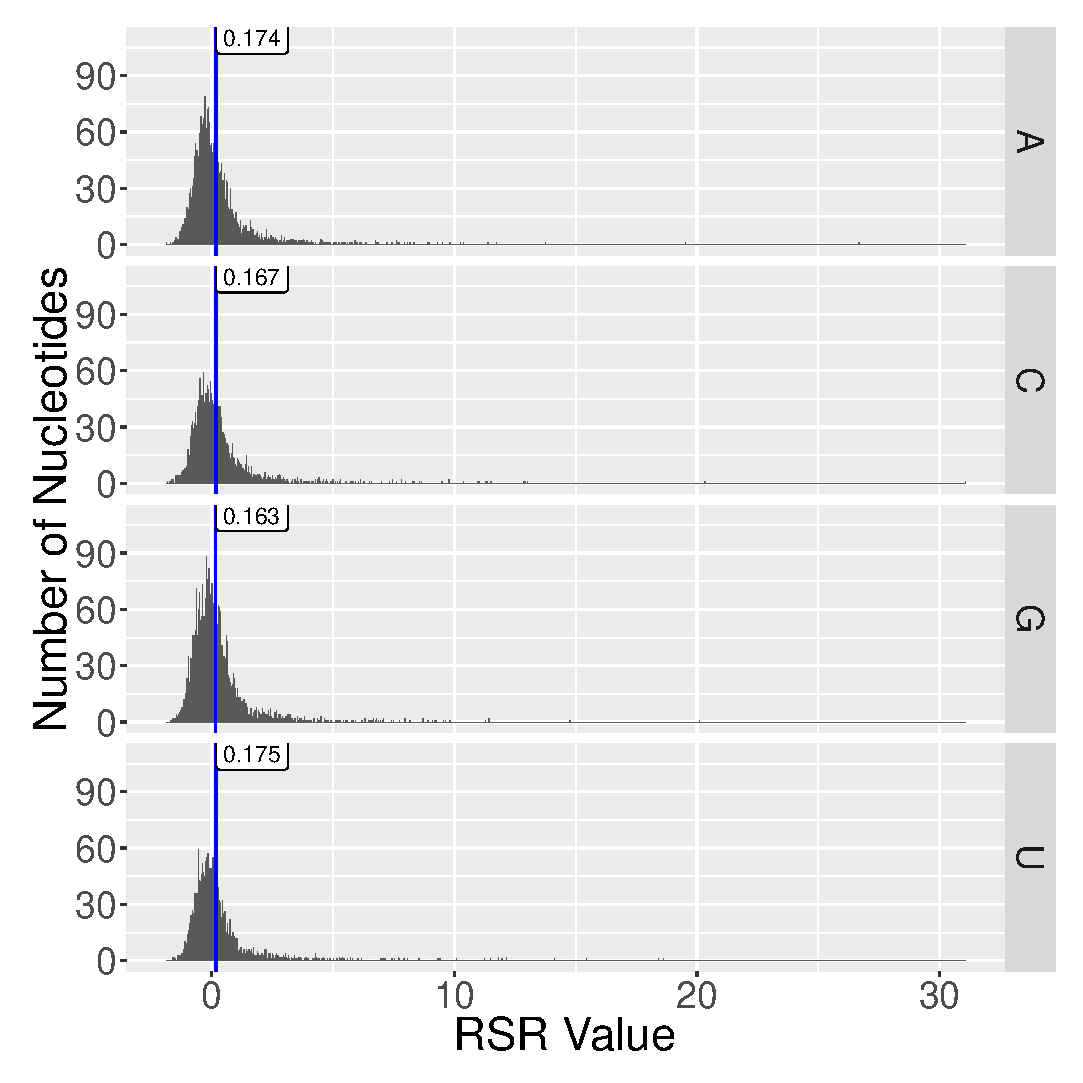
\includegraphics[width=0.5\linewidth]{chapter-5/figs/rsr-distrubutution}
  \caption{Histograms of the distribution of RSR values for nucleotides in
    loops. Each panel represents a different residue. The loop used are all
    accepted loops from Representative release 2.85. The blue bars indicate the mean
  of each distribution, while the number next to each bar shows the value of the
  mean.}
  \label{fig:rsr-nt-distribution}
\end{figure}

This figure shows that Guanine has the lowest mean RSRZ value of 0.163, while
the highest is Uracil with a mean of 0.175. These distributions have a long tail
that goes near 30, while there are few values below -1. 

There are several issues with RSR however \cite{Tickle2012}. To deal with these
issues, the corresponding Z-score, statistical measure, RSRZ, has been proposed
for general use \cite{Gore2012}. The Real Space Z-Score (RSRZ) is a normalized
version of RSR calculated by PDB. This data is calculated for each structure on
a residue level. The data is produced by computing RSR Z-Scores for each type of
residue present in the structure and comparing to like residues in all other
comparable structures of similar resolution, ie A's are compared to other A's,
while C's are compared to other C's \cite{Gore2012, Kleywegt2004a}. PDB provides
this statistic as part of their validation reports and the data is imported as
part of our weekly update pipeline. This data is available on their FTP site,
the URLs depend upon the structure, for example the data for 1FJG is available
at: \url{http://ftp.wwpdb.org/pub/pdb/validation\_reports/fj/1fjg/}. In this way
the quality of each structure is compared to other structures of comparable
resolution, as well as to all other X-ray structures in PDB that contain RNA.

\subsection{Determining how to use RSRZ to reject loops}

We begin by examining the distribution of RSRZ data for each type of loop in the
representative set of 3D structures selected as described in the previous
chapter, which corresponds to the 2.85 representative structure release
available at (\url{http://rna.bgsu.edu/rna3dhub/nrlist/release/2.85}). The
distribution of such data is shown in Figure~\ref{fig:rsrz-distribution}. In
this figure we can see that loops nucleotides have a median value near 0,
indicating a good fit to observed density. We can also see a long tail in the
RSRZ distribution that indicates a large range in the quality of modeling. PDB
assigns an RSRZ value of 2 to indicate a large outlier. This is shown on the
graphs as a red bar.

\begin{figure}
  \includegraphics[width=0.5\linewidth]{chapter-5/figs/loops/rsrz-distribution}
  \caption{Distribution of RSRZ values for nucleotides in all accepted loops.
    The nucleotides are only from loops that pass all structural criteria.}
  \label{fig:rsrz-distribution}
\end{figure}

From this distribution we can see that median value is less than 0. This
indicates that loops in bases from our representative structures are better
modeled than the average nucleotide. This supports the conclusions of the
previous chapter that appropriate criteria are used to select the representative
structure. However, there is a long tail of nucleotides with very high values.
Loops with containing poorly modeled nucleotides that should be excluded from
clustering and inclusion in the 3D Motif Atlas. I used RSRZ values to create two
criteria. The first is that all bases in a loop must be well modeled, that is
all nucleotides in the loop should have a low RSRZ value. I use this cutoff
because we want to ensure that a loop is not an ``appealing fiction'' where all
bases in it are poorly modeled. We do not consider if the bases are interacting
in this criterion because some loops do not contain interactions. Secondly, is
that all nucleotides that make interactions with other bases within the loop
must have a low RSRZ value as well. This criterion is used because we expect
that loops interacting within a loop will have a lower RSRZ value by virtue of
being ``fixed in place'' in the crystal.

\subsection{Detecting fictional loops}

The first criterion is that all bases in a loop should be sufficiently well
modeled. A well modeled base has a low RSRZ value, thus a poorly modeled loop is
one where all modeled bases in the loop have a high RSRZ value. I will refer to
these loops as ``fictional'' as they are not supported by the experimental
density. I am interested in exploring the effect of various RSRZ cutoffs on
motif clustering so we will use a range of RSRZ values. We have been advised by PDB
to implemented an RSRZ threshold of 2 to identify loops that are poorly modeled.
I tested cutoffs of 1, 1.5 and 2.5 to explore the effect of various cutoffs on
motif clustering. I applied this criterion, all nucleotides in the loop must
have an RSRZ less than the cutoff, to all valid loops in the dataset. A summary
of the number of loops sorted by this criterion into successive ranges of RSRZ
in Table~\ref{tab:cutoffs-reject-summary}.

\begin{table}
  \begin{tabular}{llrrrr}
    \toprule
              &                   & \multicolumn{4}{c}{Number of Loops Rejected by Fictional Loop Cutoff} \\
    \cmidrule(r){3-6}
    Loop Type & Total Valid Loops & \rsrz{1}  & \rsrz{1.5} & \rsrz{2} & \rsrz{2.5} \\
    \midrule
    Internal Loops & 1794 (100\%) & 19 (1\%)   & 5 (0.2\%)  & 4 (0.2\%)  & 2 (0.1\%) \\
    Hairpin Loops  & 1319 (100\%) & 45 (3.4\%) & 23 (1.7\%) & 10 (0.7\%) & 6 (0.4\%) \\
    3-Way Junction & 132 (100\%)  & 0          & 0          & 0          & 0 \\
    \bottomrule
  \end{tabular}
  \caption{Number of fictional loops according to different RSRZ cutoff values:
    Counts of the number of loops of each type rejected by the criteria that
    requires all nucleotides in a base to pass the RSRZ cutoff. The percentages
    are the percent of loops rejected out of all loops. The data is for all
    valid X-ray loops from the NR release 2.85.}
  \label{tab:cutoffs-reject-summary}
\end{table}

As expected, the lower the values of the RSRZ criterion, the more loops are
rejected. However, even for the lowest value used, RSRZ value of 1, relatively
small small number of loop instances are rejected . This is suggests that our
current set is not heavily populated with loops that do not model the data well.

% I evaluated how well structured the rejected loops are by determining the number
% of annotated interactions per nucleotide for all loops shown in
% Table~\ref{tab:all-bad-structuring}.

% \begin{table}
%   \begin{longtable}{llrrrrrr}
%   % \begin{tabulary}{\linewidth}{LlRRRRRR}
%     \toprule
%     % & & & \multicolumn{8}{c}{Number of Annotated Interactions} & & & \\
%     Loop &
%       Cutoff & 
%       Length &
%       Basepairs &
%       Stacking &
%       Base-phosphate &
%       Total &
%       Interaction Per Nt \\
%     \midrule
%     HL\_1FJG\_003 &  \rsrz{1} & 6 & 2 & 5 & 1 & 8 & 1.33 \\
%     HL\_1M5O\_004 &  \rsrz{2.5} & 6 & 1 & 4 & 1 & 24 & 4 \\
%     HL\_1ZDJ\_002 &  \rsrz{1.5} & 6 & 1 & 3 & 1 & 10 & 1.67 \\
%     HL\_1ZDJ\_004 &  \rsrz{1.5} & 6 & 1 & 3 & 1 & 10 & 1.67 \\
%     HL\_2AKE\_001 &  \rsrz{1.5} & 9 & 2 & 1 & 0 & 6 & 0.67 \\
%     HL\_2AKE\_003 &  \rsrz{1} & 9 & 2 & 5 & 1 & 8 & 0.89 \\
%     HL\_2AKE\_004 &  \rsrz{1.5} & 9 & 2 & 1 & 0 & 6 & 0.67 \\
%     HL\_2AKE\_006 &  \rsrz{1} & 9 & 2 & 5 & 1 & 8 & 0.89 \\
%     HL\_2AZX\_001 &  \rsrz{1} & 9 & 2 & 2 & 0 & 4 & 0.44 \\
%     HL\_2AZX\_010 &  \rsrz{1} & 9 & 2 & 2 & 0 & 4 & 0.44 \\
%     HL\_2CV1\_006 &  \rsrz{1} & 9 & 2 & 5 & 3 & 10 & 1.11 \\
%     HL\_2OIU\_001 &  \rsrz{1} & 6 & 2 & 5 & 0 & 7 & 1.17 \\
%     HL\_2OIU\_002 &  \rsrz{1.5} & 6 & 1 & 5 & 1 & 14 & 2.33 \\
%     HL\_2OIU\_004 &  \rsrz{1.5} & 6 & 2 & 5 & 1 & 16 & 2.67 \\
%     HL\_2OIU\_005 &  \rsrz{2.5} & 6 & 1 & 4 & 0 & 20 & 3.33 \\
%     HL\_2OIU\_006 &  \rsrz{1} & 6 & 2 & 5 & 1 & 8 & 1.33 \\
%     HL\_2VPL\_001 &  \rsrz{1} & 8 & 2 & 4 & 0 & 6 & 0.75 \\
%     HL\_3IAB\_001 &  \rsrz{1} & 6 & 2 & 5 & 1 & 8 & 1.33 \\
%     HL\_3IAB\_002 &  \rsrz{1} & 6 & 2 & 5 & 1 & 8 & 1.33 \\
%     HL\_4C9D\_002 &  \rsrz{1} & 5 & 2 & 4 & 0 & 6 & 1.2 \\
%     HL\_4DR7\_033 &  \rsrz{2.5} & 9 & 1 & 4 & 0 & 20 & 2.22 \\
%     HL\_4KR6\_001 &  \rsrz{2} & 10 & 1 & 3 & 0 & 12 & 1.2 \\
%     HL\_4KR6\_002 &  \rsrz{2} & 8 & 1 & 4 & 0 & 15 & 1.88 \\
%     HL\_4KR7\_001 &  \rsrz{2} & 6 & 1 & 3 & 0 & 12 & 2 \\
%     HL\_4KR7\_002 &  \rsrz{1.5} & 6 & 1 & 3 & 0 & 8 & 1.33 \\
%     HL\_4OO8\_005 &  \rsrz{1} & 6 & 2 & 4 & 0 & 6 & 1 \\
%     HL\_4UN5\_001 &  \rsrz{1} & 6 & 1 & 4 & 0 & 5 & 0.83 \\
%     HL\_4UYK\_003 &  \rsrz{1} & 6 & 2 & 3 & 0 & 5 & 0.83 \\
%     HL\_4V8E\_108 &  \rsrz{2.5} & 5 & 1 & 4 & 0 & 20 & 4 \\
%     HL\_4V8N\_143 &  \rsrz{1} & 12 & 2 & 2 & 1 & 5 & 0.42 \\
%     HL\_4V8P\_184 &  \rsrz{1.5} & 5 & 2 & 2 & 0 & 8 & 1.6 \\
%     HL\_4V8P\_231 &  \rsrz{1} & 8 & 1 & 5 & 0 & 6 & 0.75 \\
%     HL\_4V9F\_030 &  \rsrz{1.5} & 11 & 1 & 7 & 1 & 18 & 1.64 \\
%     HL\_4V9F\_031 &  \rsrz{1} & 8 & 1 & 6 & 1 & 8 & 1 \\
%     HL\_4V9I\_149 &  \rsrz{1} & 14 & 1 & 7 & 0 & 8 & 0.57 \\
%     HL\_4V9I\_150 &  \rsrz{1} & 9 & 2 & 7 & 1 & 10 & 1.11 \\
%     HL\_5B2S\_003 &  \rsrz{1} & 6 & 2 & 5 & 0 & 7 & 1.17 \\
%     HL\_5DM6\_030 &  \rsrz{2.5} & 5 & 1 & 2 & 0 & 12 & 2.4 \\
%     HL\_5DM6\_048 &  \rsrz{2.5} & 11 & 1 & 0 & 0 & 4 & 0.36 \\
%     HL\_5DM6\_051 &  \rsrz{2} & 10 & 1 & 3 & 0 & 12 & 1.2 \\
%     HL\_5F9R\_001 &  \rsrz{1.5} & 6 & 2 & 5 & 0 & 14 & 2.33 \\
%     HL\_5J91\_161 &  \rsrz{1.5} & 11 & 2 & 7 & 1 & 20 & 1.82 \\
%     HL\_5J91\_162 &  \rsrz{1} & 8 & 2 & 7 & 1 & 10 & 1.25 \\
%     HL\_5J91\_176 &  \rsrz{1.5} & 4 & 1 & 2 & 0 & 6 & 1.5 \\
%     HL\_5J91\_185 &  \rsrz{1.5} & 6 & 1 & 2 & 0 & 6 & 1 \\
%     IL\_1FJG\_046 &  \rsrz{1} & 5 & 2 & 3 & 0 & 5 & 1 \\
%     IL\_2IZN\_001 &  \rsrz{1} & 5 & 2 & 3 & 0 & 5 & 1 \\
%     IL\_2IZN\_003 &  \rsrz{1} & 5 & 2 & 3 & 0 & 5 & 1 \\
%     IL\_2OIU\_001 &  \rsrz{1} & 5 & 2 & 2 & 0 & 4 & 0.8 \\
%     IL\_2OIU\_002 &  \rsrz{1} & 14 & 3 & 12 & 0 & 15 & 1.07 \\
%     IL\_2OIU\_004 &  \rsrz{1} & 12 & 4 & 9 & 0 & 13 & 1.08 \\
%     IL\_3SYW\_002 &  \rsrz{1} & 6 & 2 & 6 & 0 & 8 & 1.33 \\
%     IL\_3SYW\_005 &  \rsrz{1} & 6 & 2 & 6 & 0 & 8 & 1.33 \\
%     IL\_3SYW\_008 &  \rsrz{1} & 6 & 2 & 6 & 0 & 8 & 1.33 \\
%     IL\_4V84\_259 &  \rsrz{1} & 7 & 2 & 6 & 0 & 8 & 1.14 \\
%     IL\_4V84\_260 &  \rsrz{1} & 6 & 2 & 4 & 0 & 6 & 1 \\
%     IL\_4V8P\_400 &  \rsrz{1} & 6 & 2 & 5 & 0 & 7 & 1.17 \\
%     IL\_4V9F\_078 &  \rsrz{2.5} & 6 & 2 & 5 & 0 & 28 & 4.67 \\
%     IL\_5DM6\_083 &  \rsrz{2} & 6 & 2 & 3 & 0 & 15 & 2.5 \\
%     IL\_5DM6\_088 &  \rsrz{2} & 10 & 2 & 4 & 0 & 18 & 1.8 \\
%     IL\_5J91\_276 &  \rsrz{2.5} & 5 & 2 & 3 & 0 & 20 & 4 \\
%     IL\_5J91\_310 &  \rsrz{1} & 5 & 2 & 2 & 0 & 4 & 0.8 \\
%     IL\_5J91\_327 &  \rsrz{1} & 25 & 2 & 15 & 0 & 17 & 0.68 \\
%     IL\_5J91\_328 &  \rsrz{1.5} & 20 & 2 & 3 & 2 & 14 & 0.7 \\
%     \bottomrule
%   % \end{tabulary}
%   \end{longtable}
%   \caption{Listing of all fictional loops. This lists all loops that are
%     detected as fictional loops for any RSRZ cutoff. The largest cutoff column
%   indicates the largest RSRZ cutoff required to detect this loop as fictional.}
%   \label{tab:all-bad-structuring}
% \end{table}

% \begin{table}
%   \begin{tabular}{lllr}
%     \toprule
%     Type & Cutoff     & Count & Mean Interactions per Nucleotide \\
%     \midrule
%     HL   & RSRZ > 1   & 22    & 0.96       \\
%     HL   & RSRZ > 1.5 & 13    & 1.61       \\
%     HL   & RSRZ > 2   & 4     & 1.57       \\
%     HL   & RSRZ > 2.5 & 6     & 2.72       \\
%     IL   & RSRZ > 1   & 14    & 1.05       \\
%     IL   & RSRZ > 1.5 & 1     & 0.7        \\
%     IL   & RSRZ > 2   & 2     & 2.15       \\
%     IL   & RSRZ > 2.5 & 2     & 4.34       \\
%     \bottomrule
%   \end{tabular}
%   \caption{Table of the mean interactions per nucleotide for loops reject at
%     each cutoff. The counts are for the loops that are rejected
%   }
% \end{table}

Manual inspection of the rejected loops shows that some appear to be poorly
structured A structured loop is one that has several annotated interactions, as
opposed to a structure loop which shows several interactions per nucleotide. An
example of a poorly structured loop is HL\_4DR7\_033 as shown in
Figure~\ref{fig:hl-4dr7-033}. All nucleotides in this loop have an RSRZ value
greater than 3. While this loop has no structural issues, the high RSRZ scores
indicate it is poorly modeled. In addition, the loop appears poorly modeled
because of the lack of interactions. These are the types of loops I expected to
reject with this method.

\begin{figure}
  \begin{subfigure}[b]{0.45\textwidth}
    \includegraphics[width=\textwidth]{chapter-5/figs/loops/HL-4DR7-033}
    \caption{HL\_4DR7\_033}
    \label{fig:hl-4dr7-033}
  \end{subfigure}
  \begin{subfigure}[b]{0.45\textwidth}
    \includegraphics[width=\textwidth]{chapter-5/figs/loops/HL-2OIU-005}
    \caption{HL\_2OIU\_005}
    \label{fig:hl-2oiu-002}
  \end{subfigure}
  \caption{3D structures of loop HL\_4DR7\_033, and HL\_2OIU\_005. These are
    both loops detected by all the fictional loop cutoff values. All nucleotides
    in HL\_4DR7\_033 have a RSRZ value greater than 3, while all of HL\_20IU\_002
    have an RSRZ value greater than 5 . 4DR7 is a \TT{} SSU solved at
    3.3\angstrom{} resolution \cite{Demirci2013} and 20IU is a ligase product
      solved at 2.6\angstrom{} resolution \cite{Robertson2007}.}
  \label{fig:fictional-loops}
\end{figure}

Others loops, such as HL\_2OIU\_002 as shown in Figure~\ref{fig:hl-2oiu-002},
appear to be well structured loops but poorly modeled. We believe this is
because the modeling procedure for a new structure is to begin with a previous
structures and modify parts to better fit the data. In some regions the old is
not modified enough to fit the data, or new experiment has no density in this
region. This leads to the creation of an ‘appealing fiction’, where the
structure appears reasonable but it is not experimental supported.

\subsection{Detection of loops containing poorly modeled interacting nucleotides}

The next use for RSRZ is to explore if the relationship between RSRZ values and
the number of of annotated interactions. We expect that nucleotides that are
making more interactions will have a lower RSRZ score than nucleotides that make
fewer interactions. This is because the lack of interactions may allow the base
to adopt a variety of conformations in the crystal, leading to diffuse electron
density. With diffuse data any single modeled position fits experimental
electron density poorly resulting in a high RSRZ value.

I explored this by plotting the distribution of RSRZ values for all nucleotides
in loops vs the number of FR3D annotated interactions the BGSU database records
for each nucleotide as shown in Figure NT RSRZ DIST. This figure is a 'violin
plot', which were originally developed in \cite{Hintze1998}. The figure is a mix
of a density estimation and a box plot. In this figure all nucleotides making
the same number of interactions are grouped together and a density estimate for
each group is produced. The estimate is plotted along each row and is referred
to as a ``density trace'' or ``trace'' for this description. The range of the
trace indicates the range of the values. The width of the trace at any region
indicates what fraction of all nucleotides are in this region.

In this figure I included all types of annotated interactions, base pairs, base
stacks, and base backbone interactions in the counts. This plot shows that there
is a broad range of RSRZ values for regardless of the numbers of interactions.
This range is largest for nucleotides with 0 interactions. The large range of
RSRZ values makes it difficult to examine the number of outliers in each group. To
alleviate this I created a truncated version of this plot to visualize the
number of outliers for each number of interactions as shown in
Figure~\ref{fig:truncated-rsrz-dist}. In this figure the RSRZ values are
truncated at a value of 3. Thus all nucleotides with an RSRZ value above 3 was
set to 3.

From this more focused figure we can see that there are far fewer RSRZ outliers
for nucleotides forming three or more annotated interactions (the tails are
skinnier as interactions increase) across all loop types. Another useful
detailed examination of this data is shown in Table~\ref{tab:rsrz-by-interaction-means}.
This table shows the mean and standard deviation of all distributions shown in
Figure~\ref{fig:truncated-rsrz-dist}.

This table shows that highest median value occurs with bases that make no
interactions, and this gently decrease as the number of interactions increase.
The RSRZ value for nucleotides in internal loops with zero interactions is $0.63
\pm 1.68$ , while for 3 it is $-0.02 \pm 0.74$ as shown in
Table~\ref{tab:rsrz-by-interaction-means}. This means that bases that make
interactions are both generally less well modeled, mean of 0.63 vs -0.02, and
have a much higher variability in their modeling, standard deviation of 1.68 vs
0.74.

\begin{figure}
  \begin{subfigure}[b]{0.45\textwidth}
    \includegraphics[width=\textwidth]{chapter-5/figs/loops/a}
    \caption{Violin plot of the RSRZ distribution.}
    \label{fig:rsrz-dist}
  \end{subfigure}
  ~
  \begin{subfigure}[b]{0.45\textwidth}
    \includegraphics[width=\textwidth]{chapter-5/figs/loops/b}
    \caption{Truncated violin plot}
    \label{fig:truncated-rsrz-dist}
  \end{subfigure}

  \caption{Distribution of RSRZ values for nucleotides in loops clustered by
    the total number of annotated interactions they form with other nucleotides
    in the loop. The nucleotides come from loops which pass the fictional loop
    cutoff of 1. The nucleotides are grouped by the total number of annotated interactions
    formed, including basepairs, base backbone, and base-stacking interactions.
    The distributions of the RSRZ values are represented as violin plots. The
    blue dots and inner bars within each ``bubble'' represent the mean and
    standard deviation of the data respectively. In the left plot the data is
    plotted vertically to better display the trend of decreasing mean RSRZ as
    the number of interactions for each nucleotide increases. The right plot is
    the same data, however truncated at a value of 3. All RSRZ values greater than 3
    are set to three and the data is replotted. The means and standard deviations
  are computed using the original data.}
\end{figure}

\begin{table}
  \begin{tabulary}{\linewidth}{LRRRRRRR}
    \toprule
              & \multicolumn{7}{c}{Number of Interactions} \\
    \cmidrule(r){2-8}
    Loop Type            & 0 & 1 & 2 & 3 & 4 & 5 & 6 \\
    \midrule
    Hairpin Loop & 0.73 (1.76) & 0.2 (1.04) & 0.03 (0.86) & 0.02 (0.82) & -0.05 (0.72) & -0.04 (0.48) & -0.08 (0.71) \\
    Internal Loop & 0.63 (1.68) & 0.11 (1.05) & -0.02 (0.82) & -0.02 (0.74) & -0.03 (0.63) & 0.02 (0.62) & 0.07 (0.48) \\
    3-Way Junction Loop & 0.17 (0.68) & 0.1 (0.66) & -0.02 (0.65) & -0.09 (0.6) & -0.12 (0.59) & -0.04 (0.61) & -0.15 (0.32) \\
    \bottomrule
  \end{tabulary}
  \caption{Table showing the mean and standard deviation of RSRZ for nucleotides
    in Internal, Hairpin and 3-Way Junction Loops by the number of interactions
  each nucleotide makes. The numbers in parenthesis are the standard deviation.}
  \label{tab:rsrz-by-interaction-means}
\end{table}

These observations generally confirm the expectation that nucleotides with
interactions have lower mean RSRZ values and fewer outliers. Thus I implemented
an additional criterion, that all interacting bases in a loop must have RSRZ
values below a cutoff for the loop to be included. I refer to this criterion as
the 'Interacting Nt' criterion. As with the previous criterion it is necessary
to determine its effect on clustering the effect on clustering. Shown in
Table~ref{tab:interacting-cutoff} is a summary of the number of loops excluded
by this method for each cutoff value. In other words, a loop is excluded if one
or more interacting nucleotides has RSRZ \textgreater the threshold.

\begin{table}
  \begin{tabulary}{\linewidth}{LLCCCC}
    \toprule
              &                   & \multicolumn{4}{c}{Number of Loops Rejected by Interacting Nt Cutoff} \\
    \cmidrule(r){3-6}
      Loop Type & Total Valid Loops & \rsrz{1} & \rsrz{1.5} & \rsrz{2} & \rsrz{2.5} \\
    \midrule
    Internal Loops & 1794 (100\%) & 419 (23\%)   & 239 (13\%)  & 149 (8\%)  & 92 (5\%) \\
    Hairpin Loops  & 1319 (100\%) & 430 (33\%)   & 279 (21\%)  & 198 (14\%) & 144 (11\%) \\
    3-Way Junction & 132 (100\%)  & 37 (28\%)    & 21 (16\%)   & 7 (5\%)    & 5 (4\%)\\
    \bottomrule
  \end{tabulary}
  \caption{Counts and percent of all loops extracted that are rejected by
    requiring all bases with annotated interactions passing each RSRZ cutoff.
    The percentages are the percent of all loops that are rejected by the
  cutoff.}
  \label{tab:interacting-cutoff}
\end{table}

As before increasing the RSRZ cutoff decreases the number of loops excluded.
Here we can see a much larger effect of this criterion. The highest number of
loops excluded, 400, occurs for internal loops with a constraint of RSRZ \textgreater 1, on
the other hand, the largest number of loops rejected for the previous constraint
is 45 for hairpin loops at RSRZ \textgreater 1.

We use the two criteria described here to build a new RSRZ quality assurance
step for loops; all nucleotides in a loop must have an RSRZ value below the
first cutoff value and all interacting bases must have the RSRZ below the second
cutoff value to be accepted. I use a range of cutoffs, 1, 1.5, 2, and 2.5 to
explore the effect on number of loops excluded. For the study here I used the
same RSRZ value for both cutoffs. The total number of loops rejected by this
method are summarized in Table~\ref{tab:rsrz-reject-summary}.

\begin{table}
  \begin{tabular}{llrrrrrrrr}
    Type of Motif &
      Number of Motifs &
      Number of Loops
      Number of Loops
  \end{tabular}
  \caption{Counts and percent of all loops extracted that are rejected by the
    RSRZ tested here. The percentages are the percent of all loops that are
  rejected by the cutoff.}
  \label{tab:rsrz-reject-summary}
\end{table}

I then tested the effects of all RSRZ cutoffs on the number of internal and
hairpin loops that are excluded, as shown in
Table~\ref{tab:il-rsrz-cutoffs-combinations} and
Table~\ref{tab:hl-rsrz-cutoffs-combinations}. From these tables we can see that
the

\begin{table}
  \begin{tabular}{llcccccc}
    \toprule
                                    &            & \multicolumn{5}{c}{Fictional Internal Loop Cutoff}    \\
                                                \cmidrule(r){3-7}
                                    &            & None & \rsrz{1} & \rsrz{1.5} & \rsrz{2} & \rsrz{2.5} \\
    \midrule
    \multirow{5}{*}{Interacting NT} & None       & (1945) & 19       & 5          & 4        & 2   \\
                                    & \rsrz{1}   & 372    & 372      & 372        & 372      & 372 \\
                                    & \rsrz{1.5} & 212    & 212      & 212        & 212      & 212 \\
                                    & \rsrz{2}   & 132    & 132      & 132        & 132      & 132 \\
                                    & \rsrz{2.5} & 87     & 87       & 87         & 87       & 87  \\
    \bottomrule
  \end{tabular}
  \caption{Table showing the number of Internal Loops that are rejected based
    upon the fictional loop and poorly modeled interacting nucleotides. The
    values in the cells indicate the number of loops that are rejected at each
    cutoff, with the exception of the entry in parenthesis, which indicates the
    total number of loops in the dataset. The row and column with the 'None'
    cutoff mean that the cutoff was not used. The cell with both cutoffs set to
    None show the total number in parenthesis.
  }
  \label{tab:il-rsrz-cutoffs-combinations}
\end{table}

\begin{table}
  \begin{tabular}{llcccccc}
    \toprule
                                    &            & \multicolumn{5}{c}{Fictional Hairpin Loop Cutoff}    \\
                                                   \cmidrule(r){3-7}
                                    &             & None    & \rsrz{1} & \rsrz{1.5} & \rsrz{2} & \rsrz{2.5} \\
    \midrule
    \multirow{5}{*}{Interacting NT} & None       & (1319)   & 45       & 23       & 10   & 6   \\
                                    & \rsrz{1}   & 385      & 385      & 385      & 385  & 385  \\
                                    & \rsrz{1.5} & 256      & 256      & 256      & 256  & 256  \\
                                    & \rsrz{2}   & 188      & 188      & 188      & 188  & 188  \\
                                    & \rsrz{2.5} & 138      & 144      & 139      & 138  & 138  \\
    \bottomrule
  \end{tabular}
  \caption{Table showing the number of Hairpin Loops that are rejected based
    upon the fictional loop and poorly modeled interacting nucleotides. The
    values in the cells indicate the number of loops that are rejected at each
    cutoff, with the exception of the entry in parenthesis, which indicates the
    total number of loops in the dataset. The row and column with the 'None'
    cutoff mean that the cutoff was not used. The cell with both cutoffs set to
    None show the total number in parenthesis.
  }
  \label{tab:hl-rsrz-cutoffs-combinations}
\end{table}

These tables show interesting differences. Notably that the majority of loops
are rejected because of poorly modeled interactions (the None column for the
fictional cutoff is normally the values in all other columns). However, there
are a few hairpin loops which are detected as fictional but are not detected
with the poorly modeled interaction criterion (The columns with a fictional
cutoff of 1 and interacting cutoff of 2 or 2.5). I interpret this to mean that
even in a poorly modeled loop there is at least one base making an interaction,
which allows the loop to be rejected by both criteria.

Using these tables I set the value of the two RSRZ cutoffs, so that fictional
loops are detected and excluded at an RSRZ cutoff of 1, while loops with poorly
modeled interactions are detected at an RSRZ cutoff of 2. This leads to the
exclusion of 132 internal loops and 188 hairpin loops from the data set.

\section{Exploring the effects of the new quality criteria on motif clustering}

To explore the effect of the new quality metrics on clustering, I built a Motif
Atlas release of internal loops using the representative release built in the
previous chapter. This clustering was used to test the effects of the effects of
new quality criteria on motif clustering. The quality criteria did not include
the RSRZ cutoffs developed above. By doing this we are able to build a motif
atlas and then examine what would happen if the loops were rejected by RSRZ
cutoffs. Doing so makes the comparisons of the resulting motif clusterings
simpler because changing the loops used will have many effects on the resulting
clustering.

I discuss the effects of the new quality criteria on the loops, followed by a
general description of the motif clustering and then discuss the effects of
applying the RSRZ cutoffs to the clustering.

\subsection{Summary of the new loop quality criteria}

In the first step in the motif clustering is to select loops that pass each
quality check. Shown in Table~\ref{tab:current-loop-quality} are the numbers of
loops from the representative IFE's from the 4.0{\AA} resolution cutoff rejected by
each criterion.

\begin{table}
  \begin{tabulary}{\linewidth}{LCCCCCCCCCC}
    \rot{Loop Type} &
      \rot{Total Loops} &
      \rot{Missing Nucleotides} &
      \rot{Abnormal Chain Number} &
      \rot{Incomplete Nucleotides} &
      \rot{Self-Complementary Internal Loop} &
      \rot{Too Many Symmetry Operators} &
      \rot{Subtotal with Flaws} &
      \rot{Modified Nucleotides} &
      \rot{cryo-EM loops} &
      \rot{Accepted Loops} \\
    \midrule
    Hairpin Loop & 2748 (100\%) & 171 (6\%) & 2 (0.07\%) & 35 (1\%)   & 0         & 27 (1\%) & 235 (9\%) & 103 (4\%) & 757 (27\%)  & 1653 (60\%) \\
    Internal Loop & 4334 (100\%) & 54 (1\%) & 6 (0.1\%)  & 20 (0.5\%) & 162 (4\%) & 55 (1\%) & 297 (7\%) & 151 (3\%) & 1951 (45\%) & 1945 (45\%) \\
    \bottomrule
  \end{tabulary}
  \caption{Counts of the loops that are rejected by each quality criteria for
  all loops that come from a representative IFE from the 2.85 representative
  release with resolution cutoff of 4.0{\AA}.}
  \label{tab:current-loop-quality}
\end{table}

From this table we can see that 151, or 3\%, internal loops are rejected on the
basis of modified nucleotides. This differs from the previous clustering where
0.9\% of loops were rejected \cite{Petrov2012}. In addition, the largest
fraction of loops, 45\%, that are rejected are due to being cryo-EM loops

\subsection{Description of the properties of the new motif atlas}

I used the loops that passed our updated quality checks, but not the new RSRZ
constraints, that were less than 15 nucleotides in length to build a motif
atlas. The additional constraint of 15 nucleotides only reduced the total number
of valid loops to 1757 from 1945 and was done to ensure the analysis completed
quickly. This clustering produced a grouping with 256 motif families. This is a
large change from the 372 motif families in the previous release. Shown in
Table~\ref{tab:loop-counts} is a summary of the number of motif families from
the release described here as compared to the previous release. The table
includes the counts of singleton motif families, families with only one
instance, and the recurrent motifs, families with more than one instance.

\begin{table}
  \begin{tabular}{lrrrrrrr}
    \toprule
                  &                                      & \multicolumn{3}{c}{Singleton Groups} & \multicolumn{3}{c}{Recurrent Groups} \\
    \cmidrule(r){3-5} \cmidrule(r){6-8}
    Motif Release &
      Motif Groups &
      Total & X-Ray & cryo-EM &
      Total & X-Ray & cryo-EM \\
    \midrule
    1.18 (December 2014) & 372 & 175 & 108 & 197 & 197 &     &   \\
    2.0 (July 2016)      & 256 & 109 & 109 & 0   & 147 & 147 & 0 \\
    \bottomrule
  \end{tabular}
  \caption{A table summarizing the number of internal loop motif groups in the
  previous motif release as compared to the new release. }
  \label{tab:loop-counts}
\end{table}

From this table we can see that the overall ratio of singleton to recurrent
groups remains relatively constant in both releases, with both clusterings being
nearly evenly split between singleton and recurrent motifs. In addition we see
that a large fraction of the previous singletons, 29\% of all motif groups
overall and 62\% of all singleton groups, come from cryo-em structures. There is
a smaller fraction of singletons now, 43\% as compared to the previous 47\%,
however, the change is fairly small.

I next examined the sizes of the motifs in the new clustering. Shown in
Figure~\ref{fig:num-motif-instances} is the size distribution in terms of number
of motif instances in all motifs motif. From this figure we can see there are 50
singleton motif groups and two groups with around 250 members.

\begin{figure}
  \includegraphics[width=0.5\linewidth]{chapter-5/figs/motifs/instances}
  \caption{Histogram of the number of motif instances in all motif groups. This
  figure shows the number of instances in all motif groups built in this chapter.}
  \label{fig:num-motif-instances}
\end{figure}

This figure shows a large spike at 1, indicating the large number of singleton
motifs in the clustering. The majority of motifs have fewer than 50 instances,
with only 2 motifs having near 250 instances.

The next consideration is the distribution of the number of nucleotides in the
motifs. Show in Figure~\ref{fig:num-motif-nucleotides} is the distribution of
the number of nucleotides in each motif.

\begin{figure}
  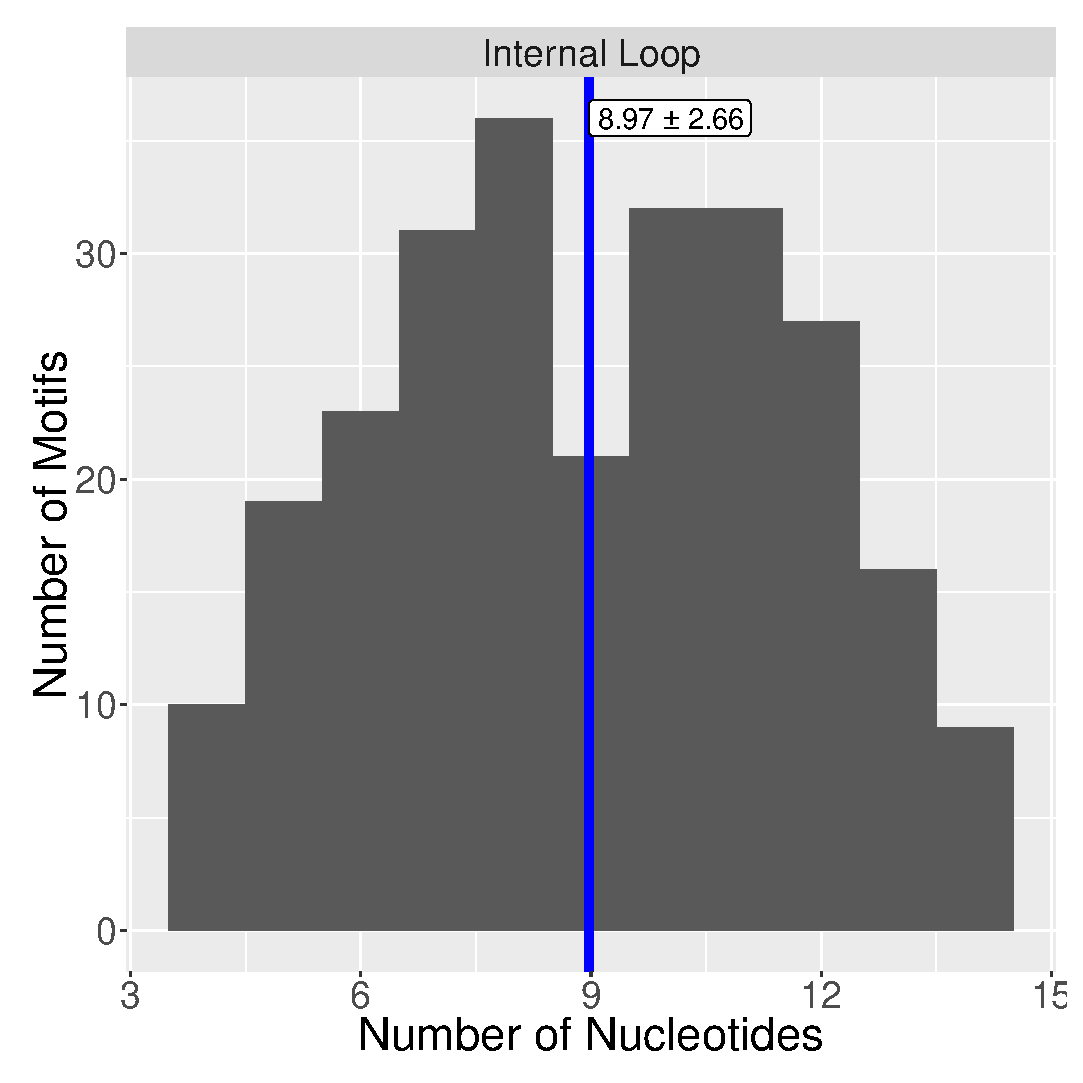
\includegraphics[width=0.5\linewidth]{chapter-5/figs/motifs/nucleotides}
  \caption{Histogram of the number of nucleotides in all motifs. This figure
  shows the counts of nucleotides in all Internal Loops in the Motif release
built in this chapter.}
  \label{fig:num-motif-nucleotides}
\end{figure}

This figure shows the overall size distribution of internal loop motifs for all
motifs in the new motif release. It is useful to know the sizes of each class of
motifs, singleton and recurrent. Shown in Figure~\ref{fig:num-nt-by-class} is this
information. This figure shows that singleton motifs tend to be larger, with a
mean of 9.5 as opposed to the mean of 8.5 for recurrent motifs.

\begin{figure}
  \includegraphics[width=0.5\linewidth]{chapter-5/figs/motifs/nucleotides-by-class}
  \caption{Histogram of the number of nucleotides in for singleton as compared
  to recurrent motifs. This figure shows the counts of nucleotides in all
  Internal Loops in the Motif release built in this chapter. The blue lines
  indicate the means of the distributions.}
  \label{fig:num-nt-by-class}
\end{figure}

\subsection{Exploration of the effects of RSRZ cutoffs on the motif clustering}

I then explored what would happen to the motif atlas when the RSRZ cutoffs
applied. This was done by examining each motif for loops that are rejected by
each RSRZ cutoff and seeing the motif would still exist. To do this I examined
what motifs in the motif atlas created above would be altered with various RSRZ
criteria. For this study I set both criteria, fictional and interacting NT, to
the same value. That is, I examined what motifs would be altered when excluding
fictional loops at an RSRZ of 1 and interacting NT's of 1 as compared to RSRZ
values of 1.5, 2, and 2.5.

I explored two main questions. First, what type of motifs are changed? Secondly,
are the loops I am removing geometrically distinct from all other loops? These
questions are explored below.

\subsubsection{What types of motifs are altered by the RSRZ criterion}

To answer the first question I explored the types of motifs, singleton or
recurrent, that would be altered for each the RSRZ criterion. Shown in
Table~\ref{tab:loop-motif-fraction} is the fraction of loops in each type of
motif that are excluded by the RSRZ cutoffs. From this table we can see that the
RSRZ criteria alter more singleton families then recurrent families. This is
most visible in the \rsrz{2.5} where while 4.7\% of all loops are rejected. If
the criterion effected singleton and recurrent motifs equally then I would
expect to see a roughly 4.7\% of singleton and recurrent motif instances being
rejected. However, what happens is that 4.3\% of loops in recurrent motifs are
rejected while 11.0\% of loops in singleton motifs are rejected. This indicates
that the singleton instances are dispositionally rejected as compared to
recurrent instances.

\begin{table}
  \begin{tabulary}{\linewidth}{LLrrrr}
  \toprule
  & & \multicolumn{4}{c}{Number of Internal Loops Excluded at} \\
        \cmidrule(r){3-6}
  Motif Type & Total Instances & \rsrz{1}     & \rsrz{1.5}   & \rsrz{2}    & \rsrz{2.5}  \\
  \midrule
  Singleton  & 109  (100\%)    & 36 (33.0\%)  & 18 (16.5\%)  & 15 (13.7\%) & 12 (11.0\%) \\
  Recurrent  & 1836 (100\%)    & 383 (20.8\%) & 221 (12.0\%) & 134 (7.2\%) & 80 (4.3\%)  \\
  Total      & 1954 (100\%)    & 419 (21.4\%) & 239 (12.2\%) & 149 (7.6\%) & 92 (4.7\%)  \\
  \bottomrule
  \end{tabulary}
  \caption{A table showing the counts of rejected loops in each type of motif,
    singleton or recurrent. The percents in the parenthesis indicate the percent
    of rejected loops that occur in each type of motif relative to all loops in
    that type of motif. Thus the upper row shows that there 109 loops in
    singleton motifs and of those 36 or 33.0\% are rejected at \rsrz{1}, while
    at \rsrz{2.5} only 12 or 11\% are rejected.}
  \label{tab:loop-motif-fraction}
\end{table}

From here I explored whether singleton or motif families are altered more
frequently by RSRZ cutoffs. Shown in Table~\ref{tab:number-motifs-altered} is
the summary of the number of motifs altered at each cutoff. From this table it
appears that the majority of motifs affected are recurrent motifs, 57\% of
recurrent motifs contain at least one loop that is rejected as compared to 33\%
percent of the singletons that contain a rejected loop. The difference between
this table, which shows that recurrent motifs are altered by RSRZ criterion, as
compared to the previous one which shows that singleton instances are altered by
RSRZ is due to the fact that there are many fewer loops that appear in a
singleton family, 109, as compared to recurrent motifs, 1685.

\begin{table}
  \begin{tabulary}{\textwidth}{lLRRR}
    \toprule
          &                   & \multicolumn{3}{c}{Number Motifs Altered} \\
                                \cmidrule(r){3-5}
    Cutoff & Number of Motifs & Total & Singletons Lost & Recurrent Altered \\
    \midrule
    \rsrz{1}   & 256 (100\%) & 120 (46\%) & 36 (14\%) & 84 (32\%) \\
    \rsrz{1.5} & 256 (100\%) & 71 (27\%)  & 18 (7\%)  & 53 (20\%) \\
    \rsrz{2}   & 256 (100\%) & 43 (17\%)  & 15 (5\%)  & 28 (10\%) \\
    \rsrz{2.5} & 256 (100\%) & 34 (13\%)  & 12 (4\%)  & 22 (9\%)  \\
    \bottomrule
  \end{tabulary}
  \caption{A table showing the number of motifs for singletons vs recurrent
    motifs with rejected loops for each cutoff tested here. The counts are the
    number of loops rejected by each cutoff while the percents in the
    parenthesis are the fraction of all motifs of that type that are are
    affected by the cutoff. The upper left column indicates that there are 120
    total motifs that contain rejected loops, and this is 46\% (120/256) of all
    motifs, while the column to the right indicates that 33\% (36/109) of all
  singleton motifs are rejected by the RSRZ \textgreater 1 cutoff.}
  \label{tab:number-motifs-altered}
\end{table}

\subsubsection{Are the loops altered distinct from other loops}

To test if the RSRZ criteria effects singleton groups more than recurrent motifs
I created a table that shows the counts of loops in each class, singleton vs
recurrent motifs that are rejected as normalized by the total number of loops
shown in Table~\ref{tab:loop-motif-fraction}. This table shows that vast
majority of rejected loops, greater than 85\% for all cutoffs, occur in
recurrent motifs. From this I infer that the singleton motifs are generally
modeled correctly. However, the recurrent motifs  often contain poorly  modeled
loops. This is consistent with the hypothesis that poorly modeled loops occur
because a structure was used as a template and a loop was not modified to fit
the new data well.

To answer the second question I created a histogram of the minimum for excluded
loops to all other loops it's motif group show in
Figure~\ref{fig:exclude-min-disc}. From this figure we can see that the RSRZ
cutoffs appear to reject outliers within groups as the distribution of
discrepancy values peaks near 0, indicating that there is always at least one
other loop that the outlier is similar to.

\begin{figure}
  % \includegraphics[width=0.5\linewidth]{chapter-5/figs/discrepancies}
  \caption{A histogram of the minimum discrepancy from a rejected loop to all
    other loops in the motif family. Lower values indicate a more similar pair
    of instances. Our motif atlas requires that all instances in the same motif
  family have discrepancy less than 1{\AA}/nt.}
  \label{fig:exclude-min-disc}
\end{figure}

This figure shows that the excluded loops are often similar to at least one
other member of their family. This indicates that our RSRZ criteria is not
removing geometric outliers from each motif family.

The RSRZ criteria appear to primarily exclude members of recurrent motifs that
are geometrically similar to other members of the motif family. RSRZ criteria
have a much smaller effect than than other motifs, most notably the criteria to
not use any loops from cryo-em structures.

\section{Conclusions and future work}

Here I have described improvements to the previous loop selection criteria, as
well as a new method that uses a measure of modeling quality, RSRZ, to better
select loops. After investigating the effects of these new criteria on
clustering we see that the largest effect comes from rejecting loops from
cryo-em structures. Usage of RSRZ does not appear to improve the homogeneity of
groups, as seen by examining the discrepancies of rejected loops. However,

Future work may focus on exploring other measures such as number of clashes in a
motif. In addition, it is possible to calculate RSRZ by parts of nucleotides,
base separate from backbone. Doing so could provide a more refined measure of
the modeling quality.
